\documentclass{standalone}
\usepackage{tikz}

\begin{document}

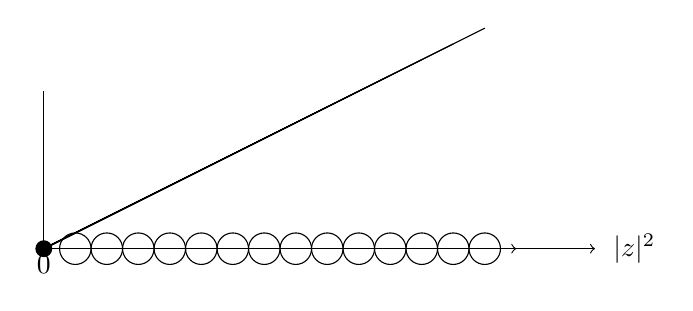
\begin{tikzpicture}[scale=2]
    % Draw the horizontal line
    \draw[->] (0,0) -- (3,0);
    
    % Label the origin
    \node at (0,-0.1) {$0$};
    
    % Draw the vertical line
    \draw (0,0) -- (0,1);
    
    % Draw the circles
    \foreach \x in {0.2,0.4,...,2.8} {
        \draw (\x,0) circle (0.1);
    }
    
    % Draw the arrow for |z|^2
    \draw[->] (3,0) -- (3.5,0);
    \node at (3.75,0) {$|z|^2$};
    
    % Draw the point at 0
    \filldraw (0,0) circle (0.05);
    
    % Draw the line from the point to the circles
    \draw (0,0) -- (0.2,0.1);
    \draw (0,0) -- (0.4,0.2);
    \draw (0,0) -- (0.6,0.3);
    \draw (0,0) -- (0.8,0.4);
    \draw (0,0) -- (1.0,0.5);
    \draw (0,0) -- (1.2,0.6);
    \draw (0,0) -- (1.4,0.7);
    \draw (0,0) -- (1.6,0.8);
    \draw (0,0) -- (1.8,0.9);
    \draw (0,0) -- (2.0,1.0);
    \draw (0,0) -- (2.2,1.1);
    \draw (0,0) -- (2.4,1.2);
    \draw (0,0) -- (2.6,1.3);
    \draw (0,0) -- (2.8,1.4);
\end{tikzpicture}

\end{document}